\chapter{Réalisation}

\section{Tableau de bord}
\centerline{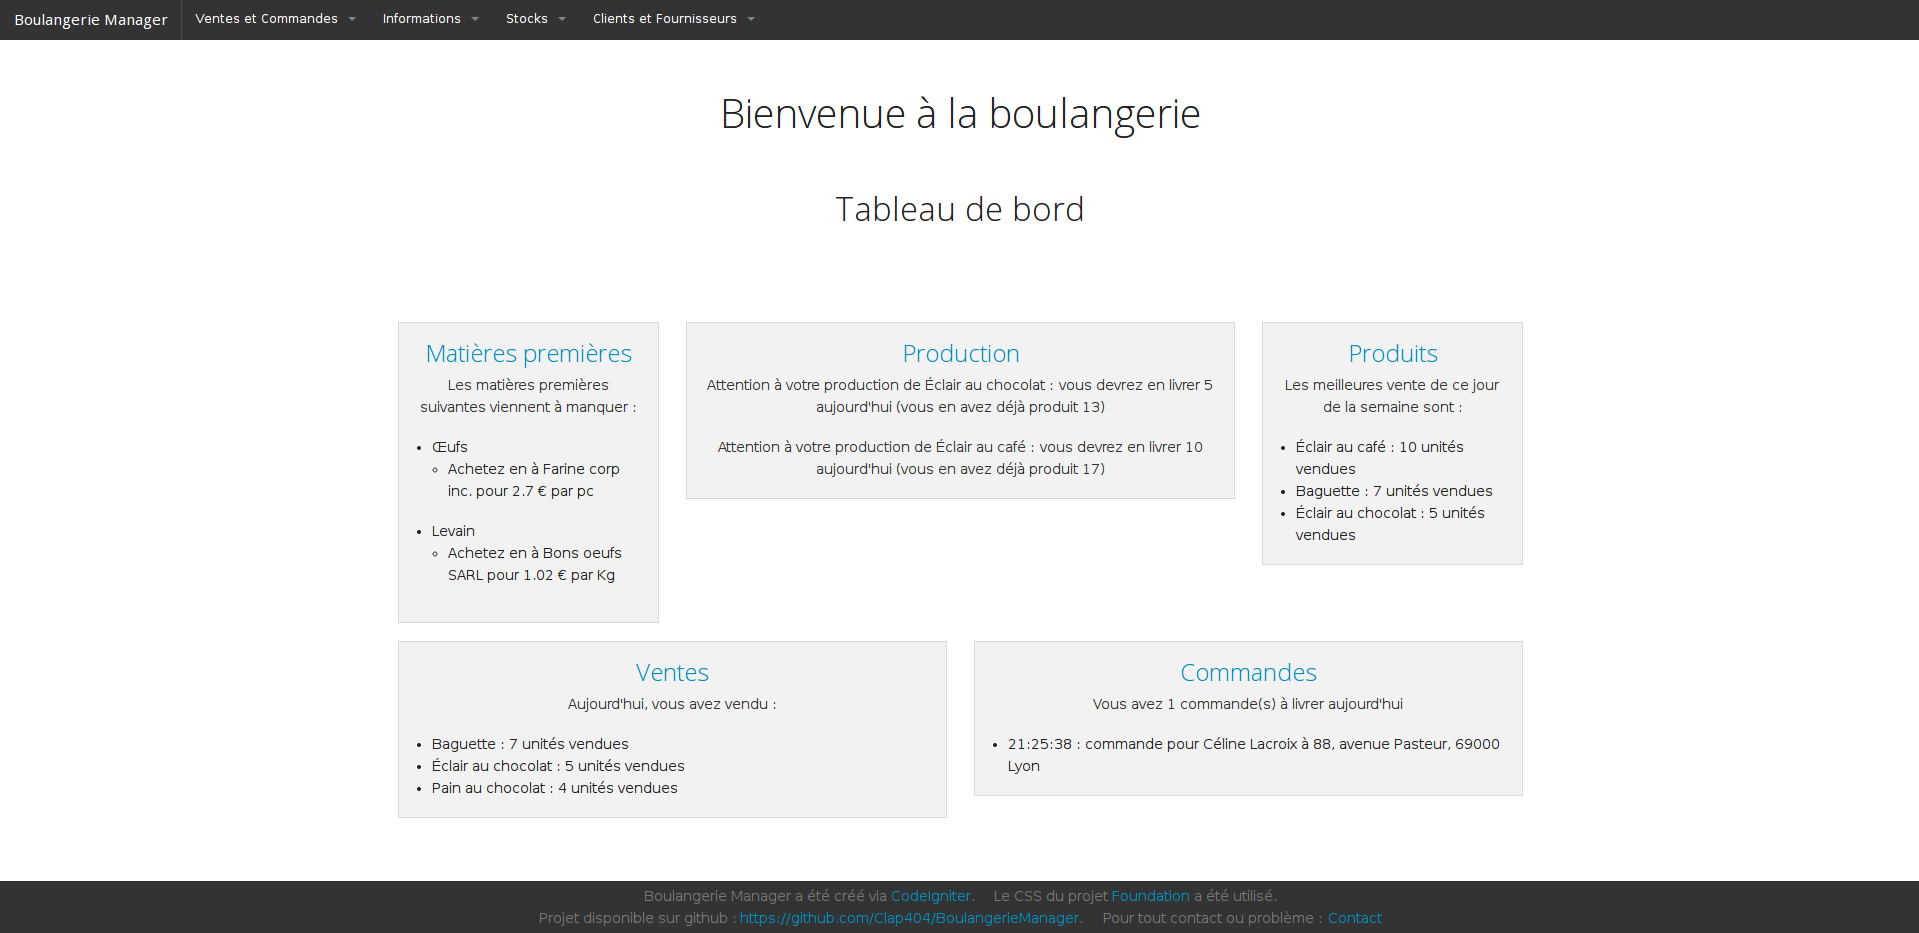
\includegraphics[width=1\textwidth]{images/tableau_de_bord.png}}
Le tableau de bord est la page d'accueil de l'application. Il montre les
informations critiques pour chaque catégorie gérée par l'application.
Les sections associées aux cadres d'information sont accessibles directement, faisant de
cette page un portail d'accès efficace.

\section{Statistiques et Invendus}
\centerline{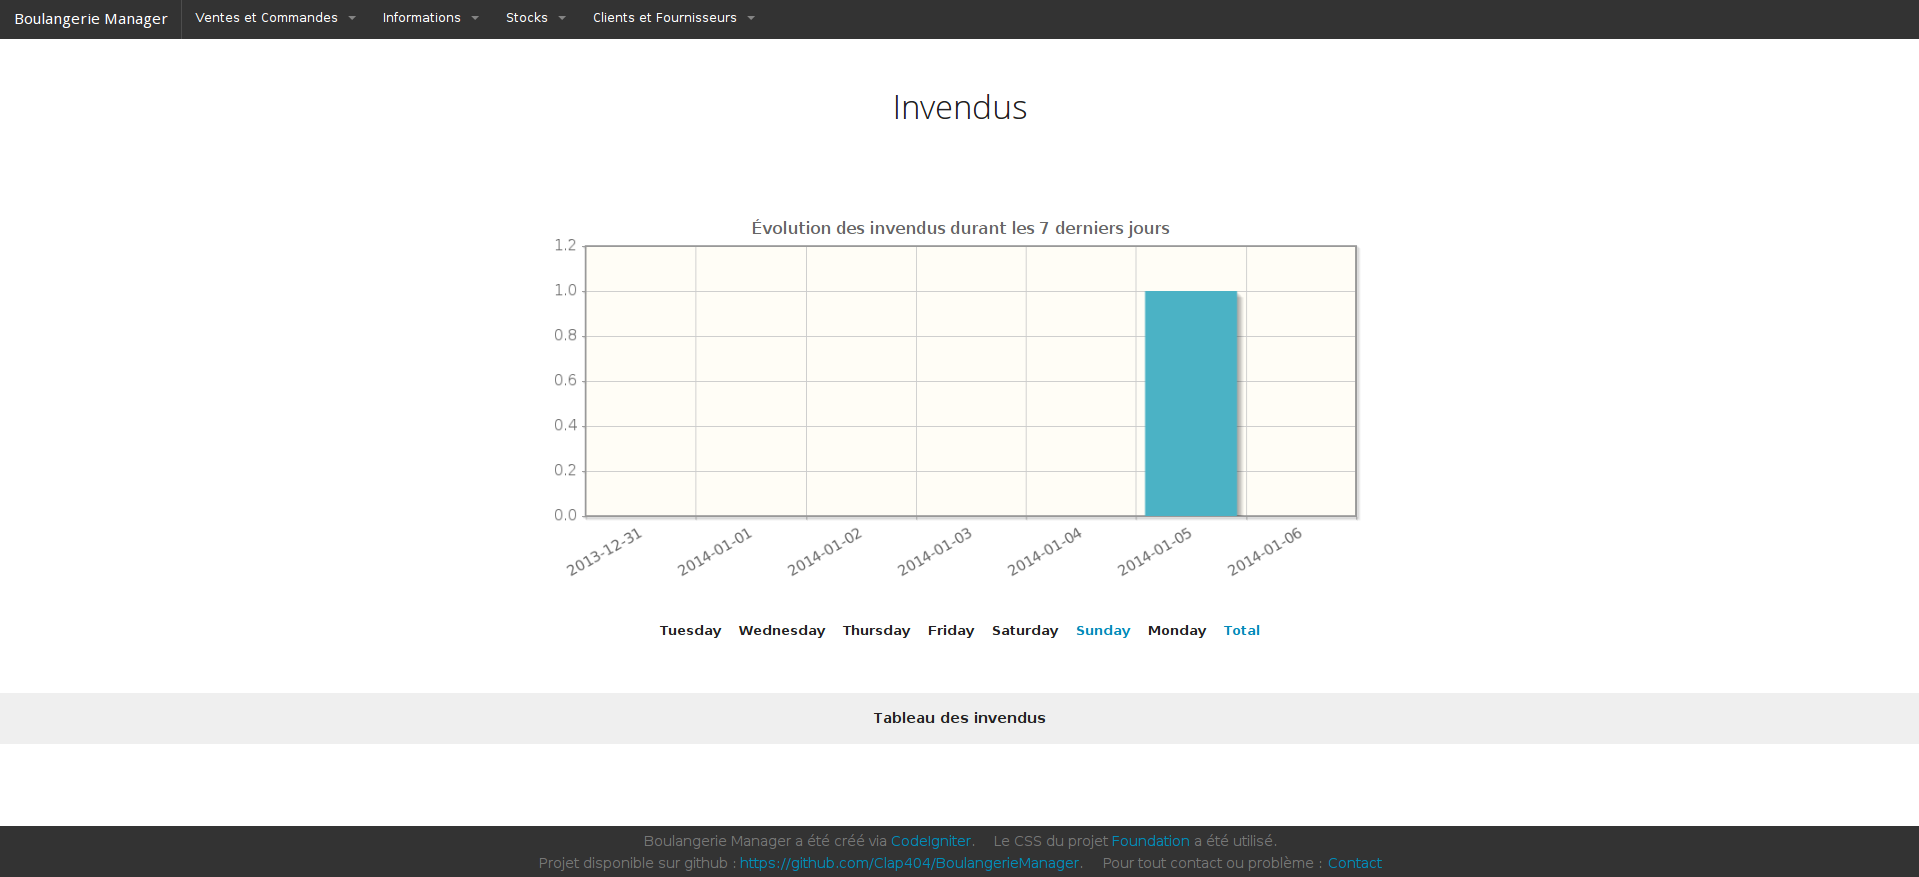
\includegraphics[width=1\textwidth]{images/Invendus.png}}
Les pages de statistique et invendus mettent l'accent sur la lisibilité en
présentant les informations sous forme de graphiques facilement analysables
par l'utilisateur.

\section{Commandes et Ventes}
\centerline{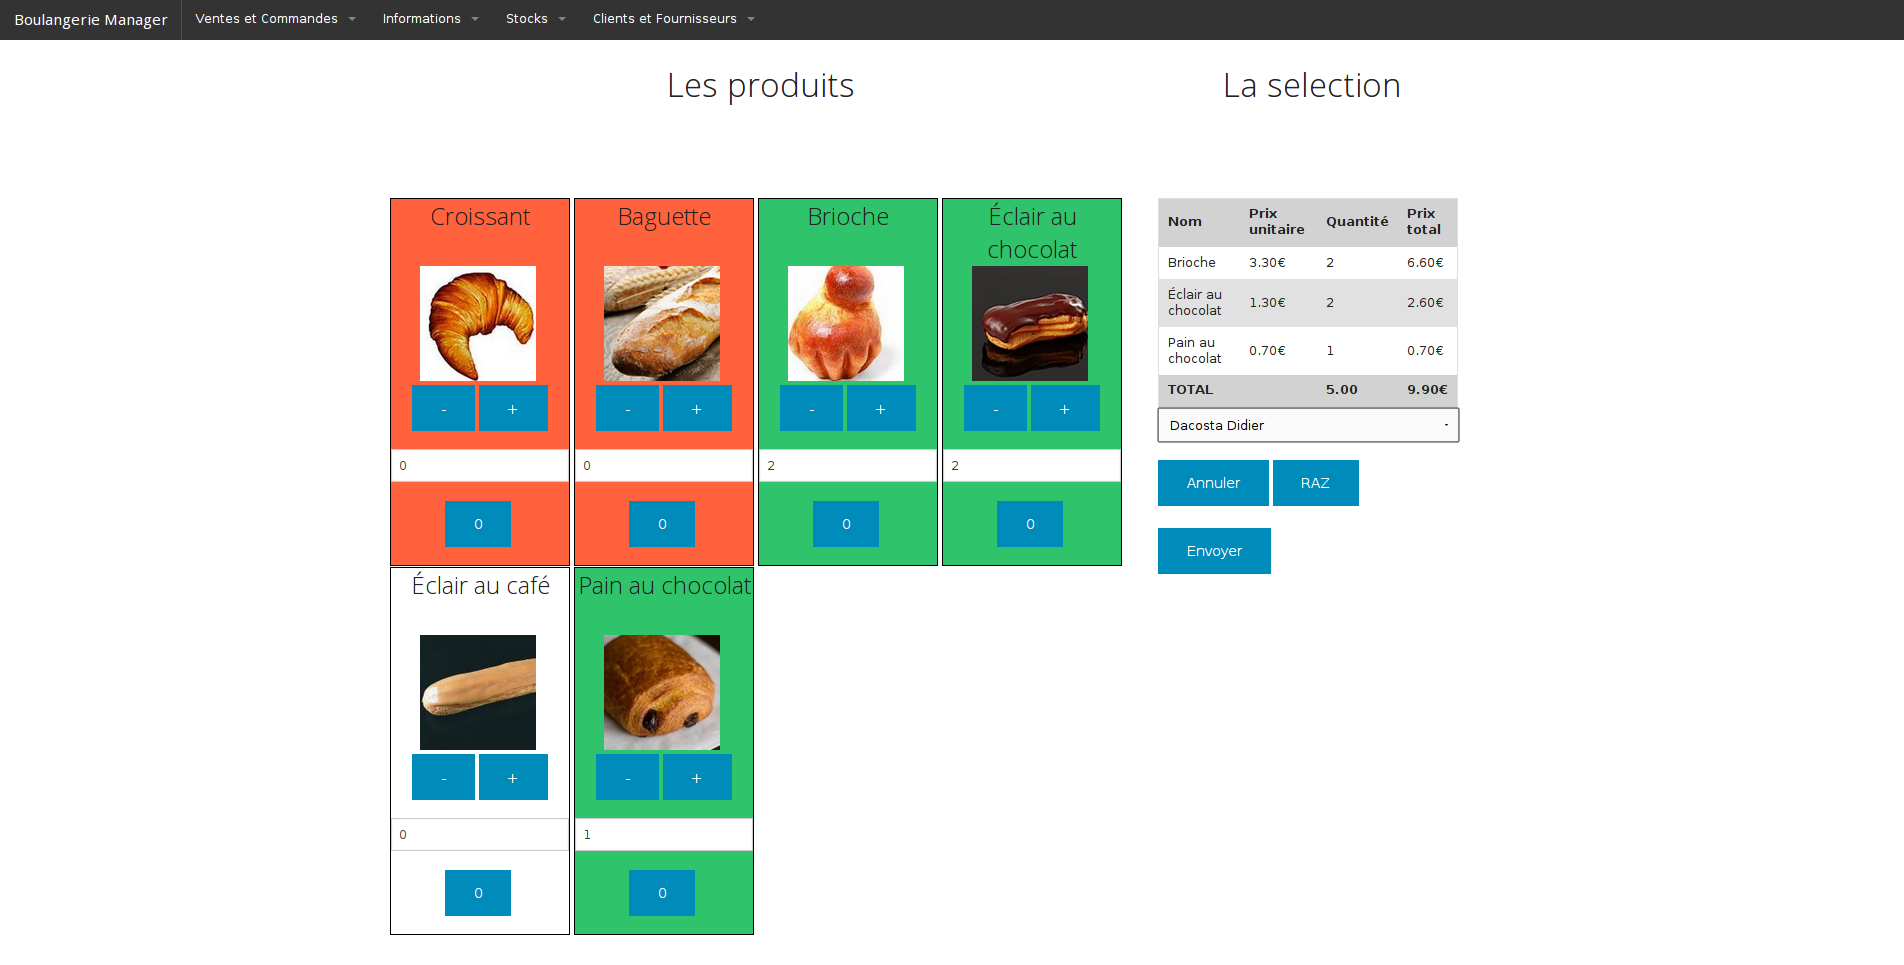
\includegraphics[width=1\textwidth]{images/ventes.png}}
L'interface utilisée pour passer de nouvelles ventes et commandes a été pensée
pour être utilisée facilement avec un écran tactile. Les images des produits
permettent de trouver rapidement le produit souhaité. Les boutons sous chaque
vignette permettent l'ajout rapide de produits. Les stocks sont pris en compte
lors de l'ajout d'une commande et signalés à l'utilisateur.

\section{Fournisseurs et Clients}
\centerline{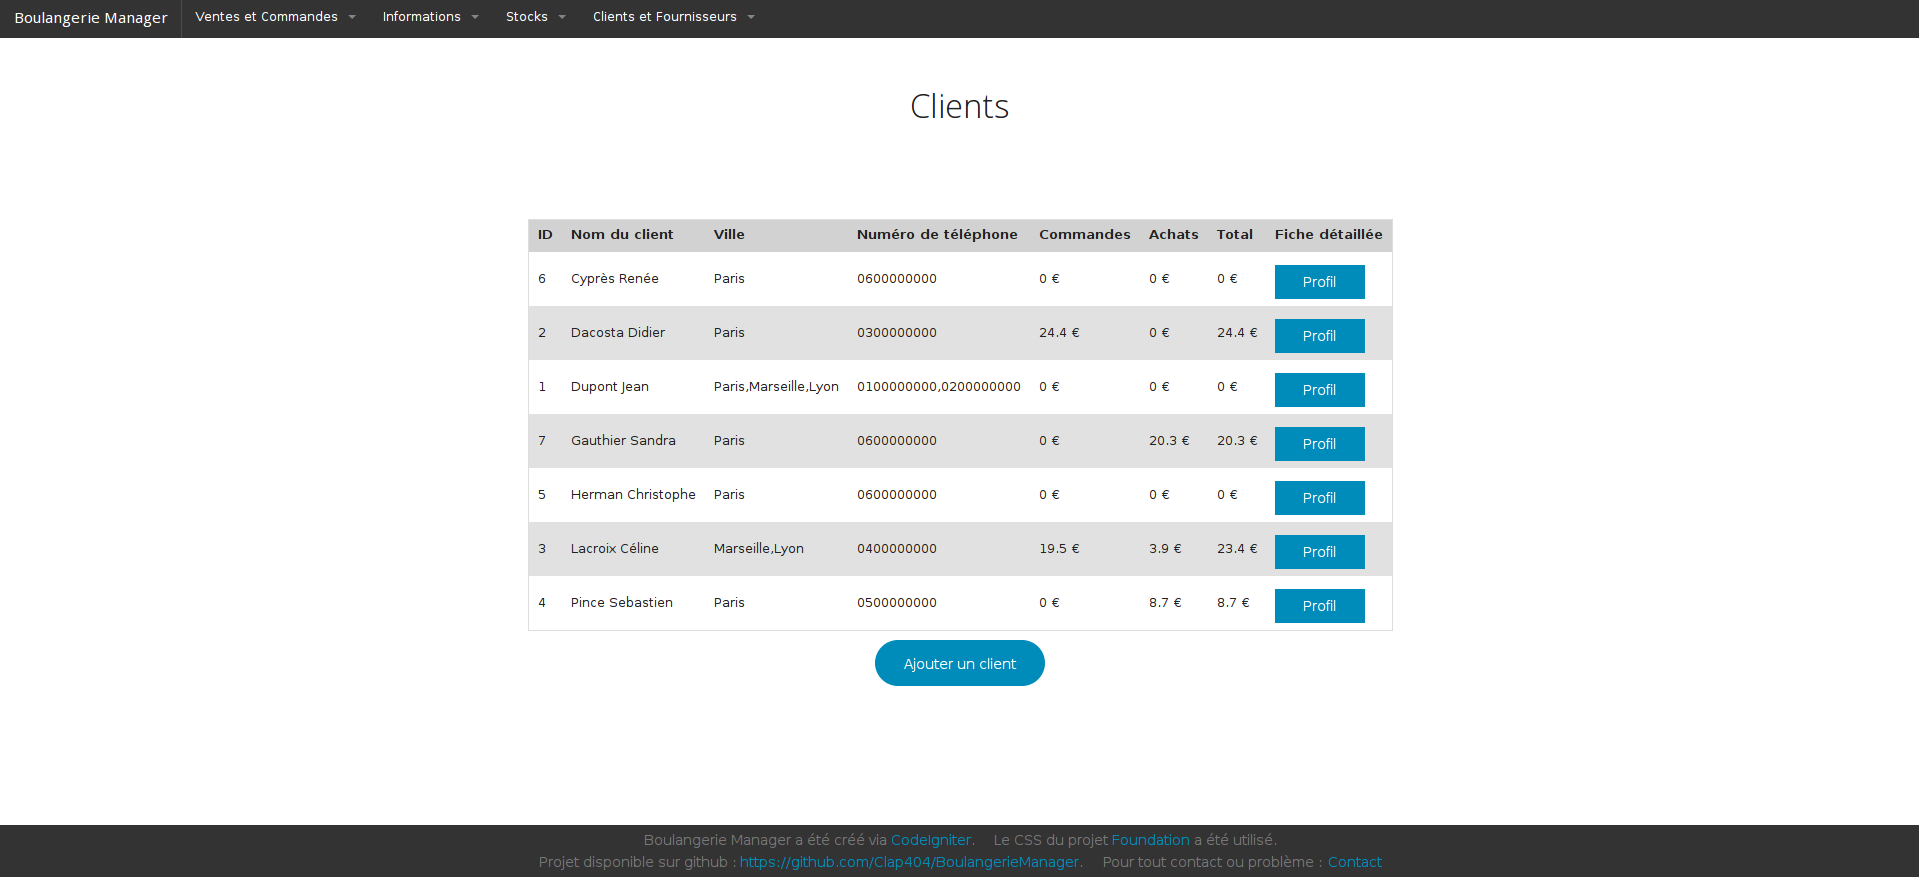
\includegraphics[width=1\textwidth]{images/clients.png}}
La gestion des clients et des fournisseurs s'effectue via une interface donnant
les informations les plus importantes directement dans la liste principale.
Pour les clients, le montant total des commandes passées est directement affiché
pour faciliter l'identification des meilleurs clients par l'utilisateur.

